\documentclass[a4paper, 12pt]{article}%тип документа

%отступы
\usepackage[left=2cm,right=2cm,top=2cm,bottom=3cm,bindingoffset=0cm]{geometry}

%Русский язык
\usepackage[T2A]{fontenc} %кодировка
\usepackage[utf8]{inputenc} %кодировка исходного кода
\usepackage[english,russian]{babel} %локализация и переносы

%Вставка картинок
\usepackage{wrapfig}
\usepackage{graphicx}
\graphicspath{{pictures/}}
\DeclareGraphicsExtensions{.pdf,.png,.jpg}

%оглавление
\usepackage{titlesec}
\titlespacing{\chapter}{0pt}{-30pt}{12pt}
\titlespacing{\section}{\parindent}{5mm}{5mm}
\titlespacing{\subsection}{\parindent}{5mm}{5mm}
\usepackage{setspace}

%Графики
\usepackage{multirow}
\usepackage{pgfplots}
\pgfplotsset{compat=1.9}

%Математика
\usepackage{amsmath, amsfonts, amssymb, amsthm, mathtools}

%Заголовок
\author{Валеев Рауф Раушанович \\
группа 825}
\title{\textbf{Работа 4.5.3\\Интерференция лазерного излучения}}
\newtheorem{task}{Задача}
\date{}
\begin{document}
\maketitle
\section*{Теория}
\subsection*{Спектр источника света}
Каждый атом может находится в одном из нескольких дискретных состояний, характеризующихся каждое своей энергией. На этом основана определение \textit{спектральной плотности излучения} $I_e(f - f_0)$.

\begin{figure}[h]
\begin{center}
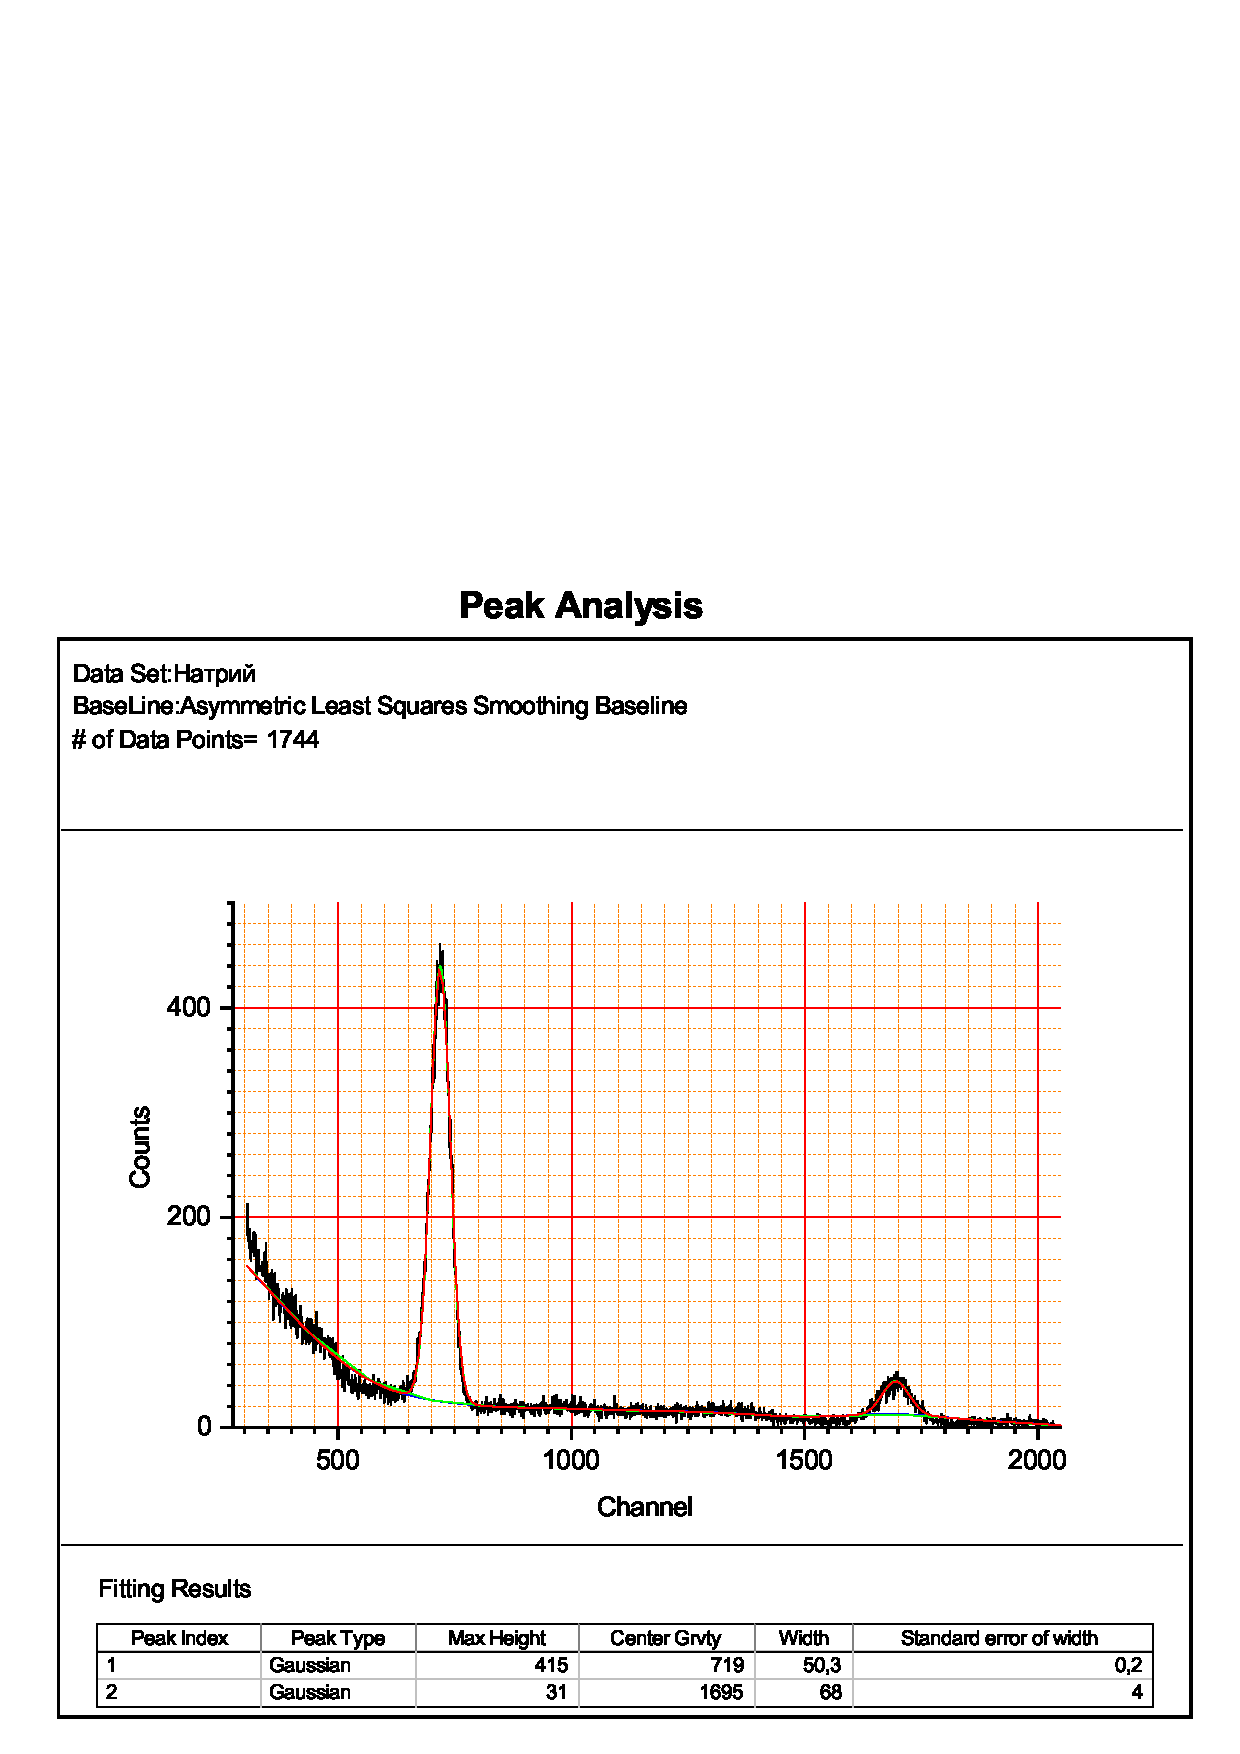
\includegraphics[width = 0.7\textwidth]{1.png}
\caption{Доплеровский контур линии излучения. Частотная характеристика резонатора и лазерные моды}
\end{center}
\end{figure}

Можно вывести, что 
\begin{equation}
I_D(f-f_0) \sim e^{-\left(\frac{\Delta f}{\Delta f_D}\right)^2}
\end{equation}

где $\Delta f = f - f_0$ и $\Delta f_D = f_0 \sqrt{\frac{2kT}{mc^2}}$

Эта функция описывает так называемый \textit{доплеровский контур линии}.
\newpage
\subsection*{Излучение $He-Ne$ лазера}

\begin{wrapfigure}{r}{0.5\textwidth}
  \begin{center}
    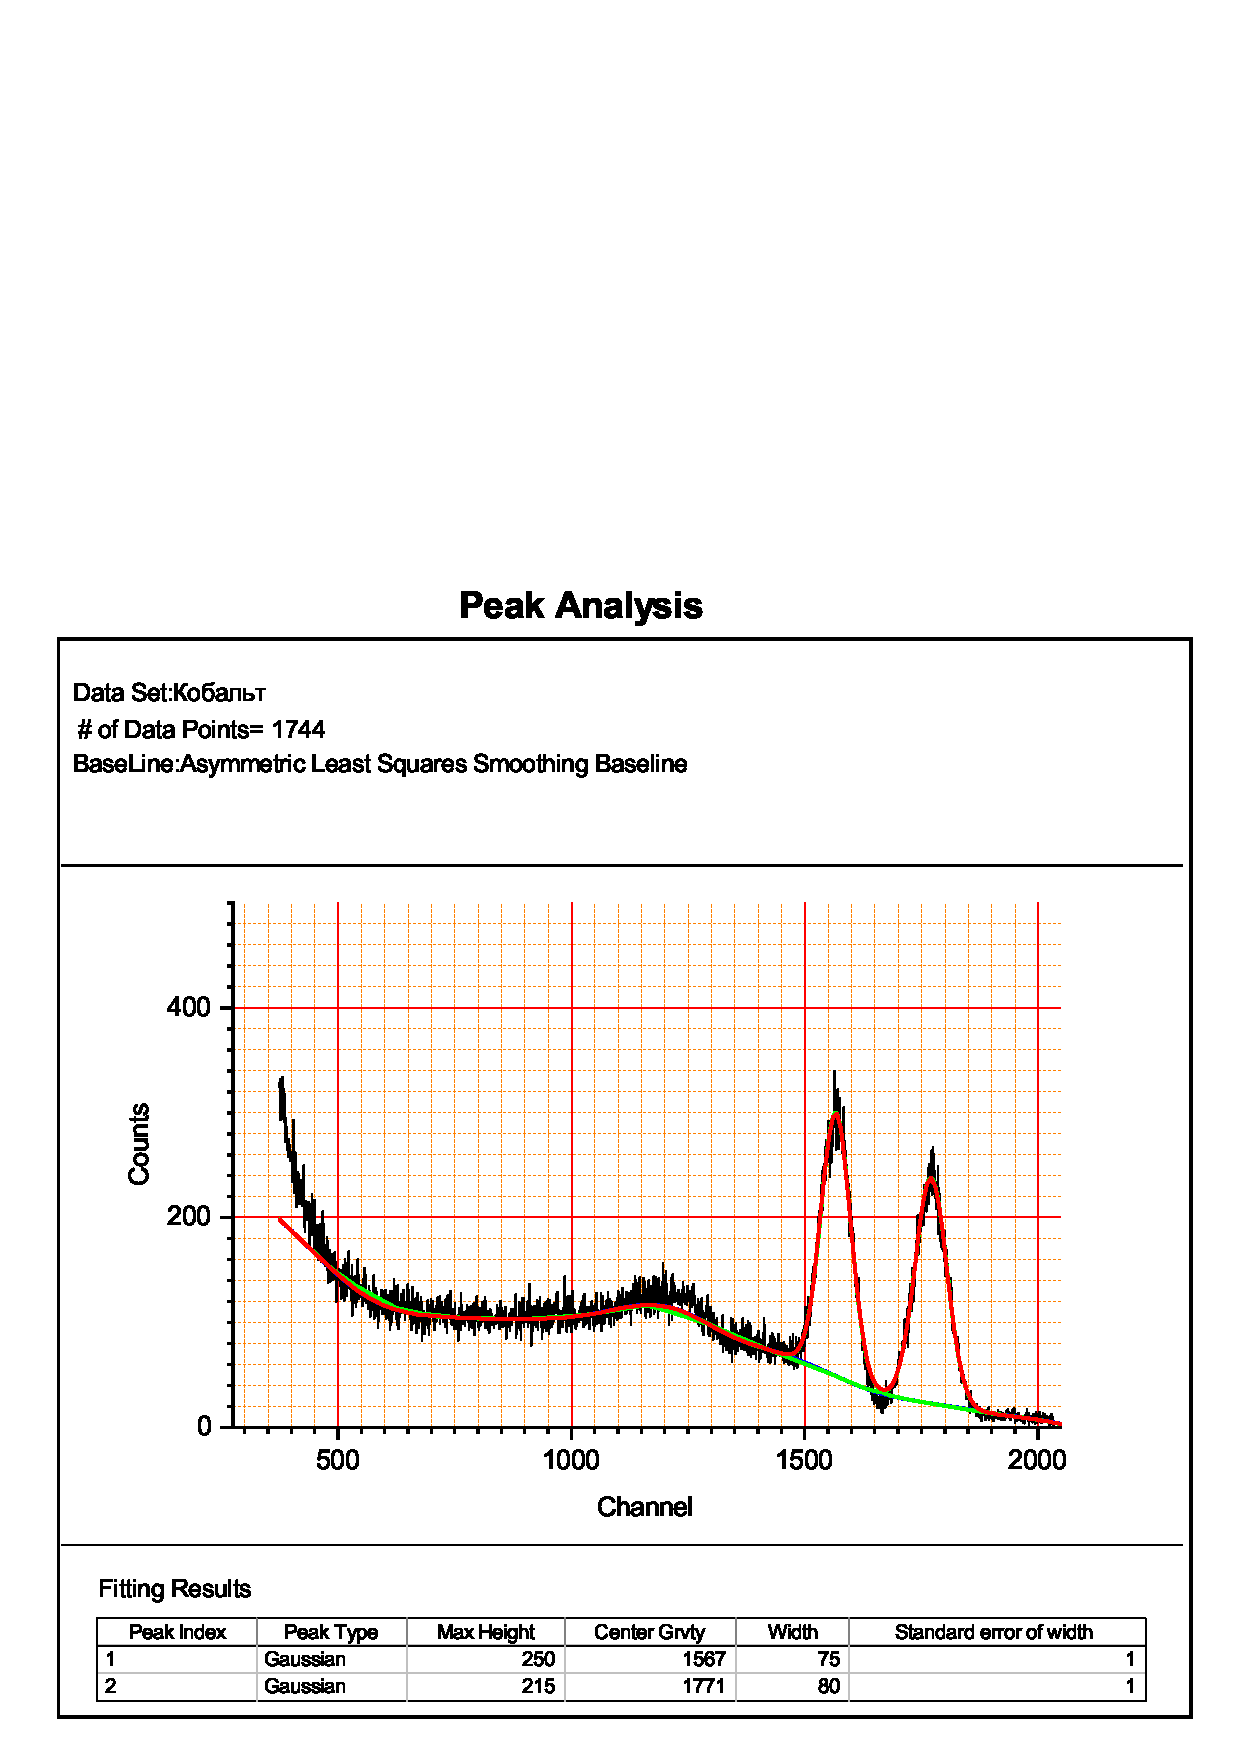
\includegraphics[width = 0.4\textwidth]{2.png}
  \end{center}
  \caption{Принципиальная схема лазера}
\end{wrapfigure}

Схема лазера приведена на рис. 2. Газоразрядная трубка $T$ наполнена смесью гелия и неона. Излучение, распространяющееся вдоль оси трубки и поляризованное в плоскости падения света, не испытывает потерь на отражение. Вследствие этого лазер генерирует линейно поляризованное излучение.

\begin{equation}
f_m = \frac{c}{\lambda_m} = \frac{mc}{2L}
\end{equation}

$(2)$ --- условие на частоты, чтобы работал интерферометр.

Рассмотрим спектральный состав излучения лазера. Условие возбуждения генерации может быть одновременно выполнено для нескольких колебаний с резонансными частотами $f_m$, в этом случае лазер будет генерировать сразу несколько световых частот с различными модами.
\begin{equation}
\Delta \nu = f_{m+1} - f_m = \frac{c}{2L}
\end{equation}

Число мод можно оценить как
\begin{equation}
N \approx 1 + \frac{2\Delta F}{\Delta \nu}
\end{equation}

\subsection*{Видность интерференционной картины}
При сложении двух когерентных световых волн возникает интерференционная картина.

\begin{equation}
\gamma = \frac{I_{\max} - I_{\min}}{I_{\max} + I_{\min}}
\end{equation}

$\gamma$ --- параметр видности, меняющийся от 0 до 1 --- самая лучшая видность.

Найдем видность для 1 моды. Легко вывести, что она равна

\begin{equation}
\gamma_1 = \frac{2 \sqrt{\delta}}{1 + \delta}
\end{equation}

где параметр
\begin{equation}
\delta = \left( \frac{B_m}{A_m}\right)^2
\end{equation}

Выражает отношение интенсивностей интерферирующих волн.

Для нескольких волн
\begin{equation}
I = \sum\limits_m I_m = \sum\limits_m A_m^2 \left[1 + \delta + 2\sqrt{\delta}\cos\left(\frac{2\pi f_m}{c}l\right)\right]
\end{equation}

\newpage
Видность всей картины 
\begin{equation}
\gamma = \gamma_1 \gamma_2(l)
\end{equation}

где

\begin{equation}
\gamma_2(l) = \dfrac{\sum\limits_n A_n^2 \cos \frac{2\pi\Delta \nu n l}{c}}{\sum\limits_n A_n^2}
\end{equation}

Причем можно получить оценку
\begin{equation}
\gamma_2 = \dfrac{\int\limits_{-\infty}^{+\infty}e^{-\left(\frac{\nu}{\Delta F}\right)^2} \cdot \cos \frac{2\pi\nu l}{c} d\nu}{\int\limits_{-\infty}^{+\infty}e^{-\left(\frac{\nu}{\Delta F}\right)^2} d\nu} = \exp\left(- \left(\frac{\pi \Delta F l}{c}\right)^2\right)
\end{equation}

\section*{Установка}
\begin{wrapfigure}{r}{0.5\textwidth}
  \begin{center}
    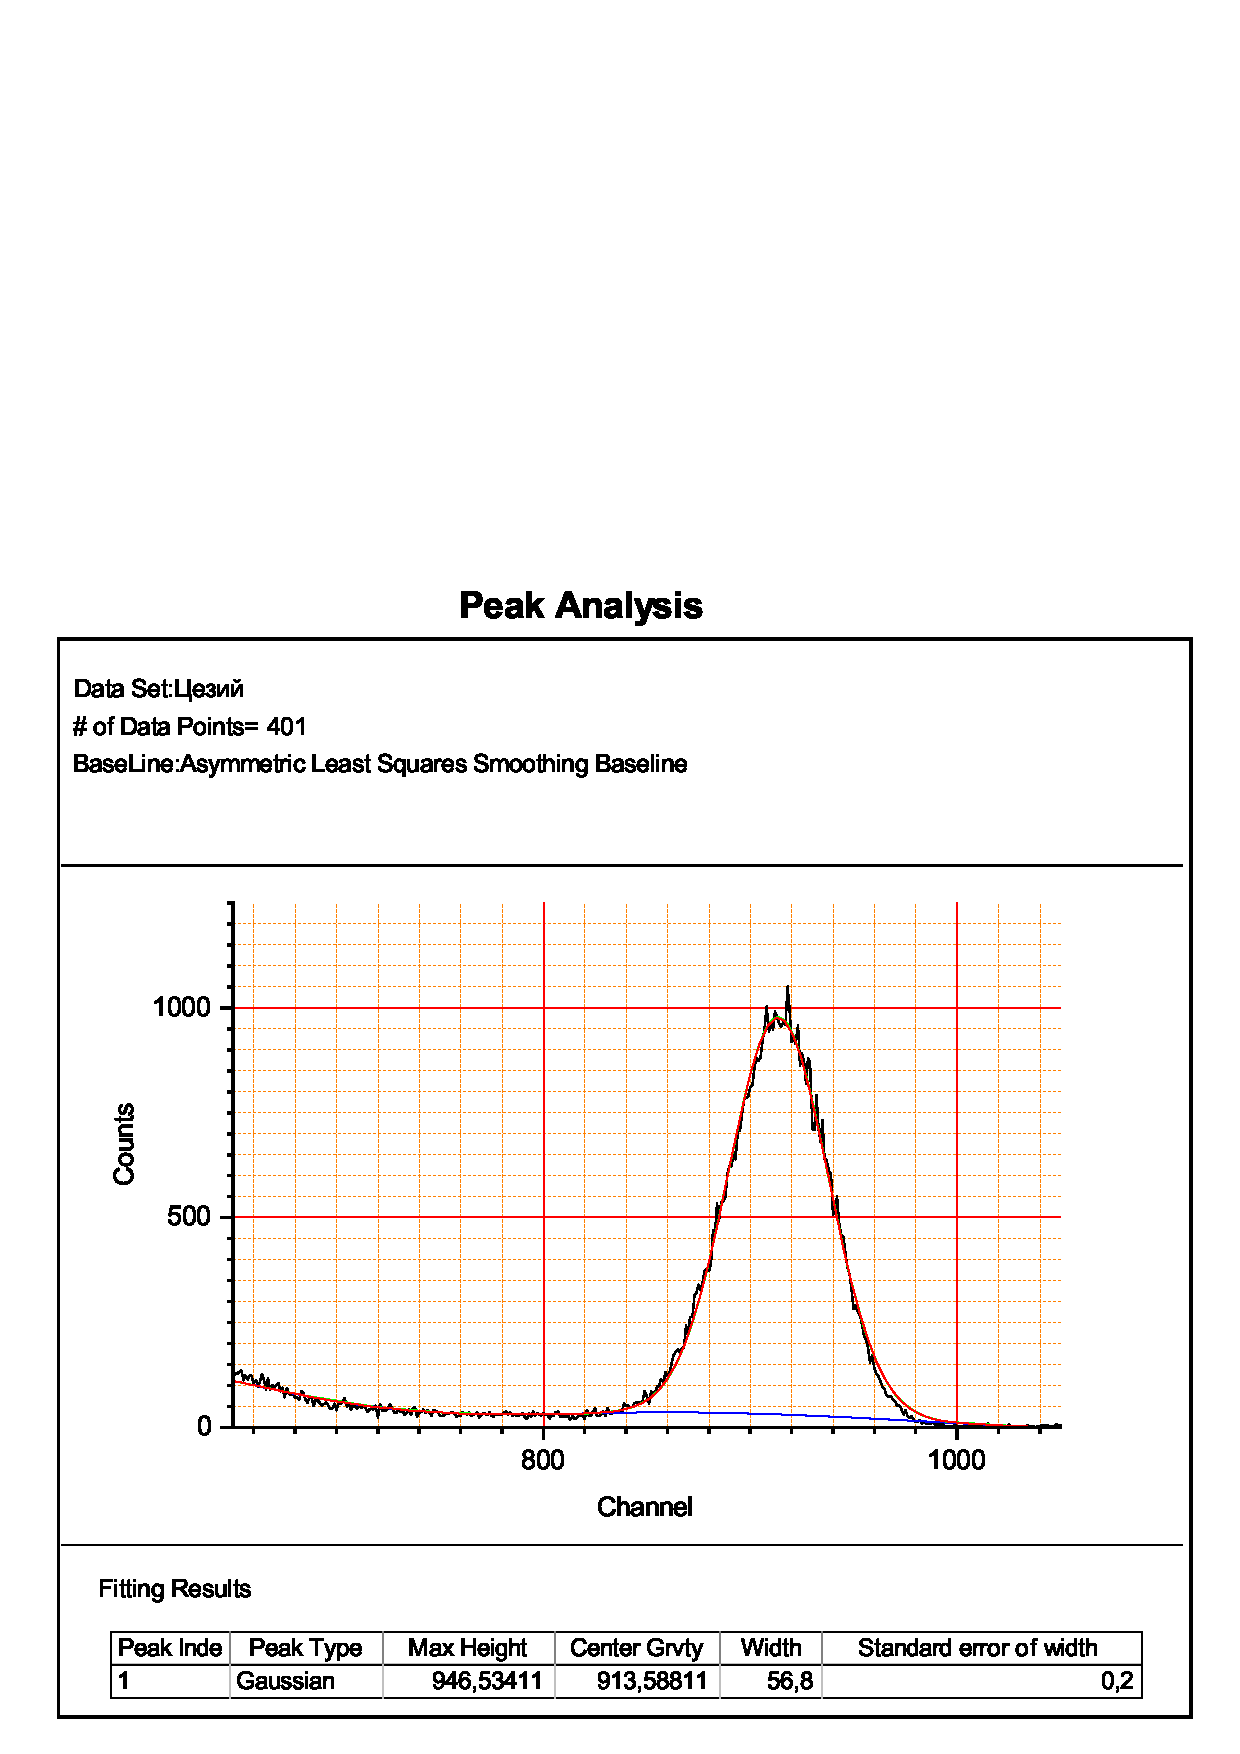
\includegraphics[width = 0.5\textwidth]{3.png}
  \end{center}
  \caption{Экспериментальная установка}
\end{wrapfigure}
Луч 1 про ходит поляроид П1, отражается под небольшим углом от зеркала З1, снова про ходит поляроид П1 и, частично отражаясь от диагональной плоскости делительной призмы, выходит из интерферометра. Зеркало З1 наклеено на пьезокерамику ПК, которая может осуществлять малые колебания зеркала вдоль падающего луча. Поляроид и зеркало с пьезокерамикой собраны в единый блок Б1, который крепится к вертикально стоящей плите.

Луч 2 проходит линзу Л, поляроид П2, отражается от зеркала З2, снова проходит поляроид П2, линзу Л и частично выводится делительной призмой из интерферометра. Зеркало З2 установлено в фокальной плоскости линзы Л. Это сделано для того, чтобы падающий и выходящий из системы лучи всегда были параллельны друг другу.
\subsection*{Настройка установки}
Луч 1, падающий на блок Б1, должен идти строго вертикально и проходить сквозь делительную призму ПД (кубик). Расстояние от вертикальной плиты до луча проверяют специальным шаблоном и при необходимости изменяют перемещением поворотного зеркала З (выполняется лаборантом). Луч 2, идущий к блоку Б2, должен идти параллельно вертикальной плите и попадать на центр линзы Л. Перекрывают луч 1 листом бумаги. Расположив блок Б2 почти вплотную к делительной призме, поворотным зеркалом подводят световое пятно к центру линзы (выполняется лаборантом). Переместив подвижный блок на дальний край штанги, совмещают пятно с центром линзы вращением кубик а вокруг вертикальной оси и горизонтальной оси, перпендикулярной плите.
\subsection*{Измерение коэффициента видности}
\begin{wrapfigure}{r}{0.3\textwidth}
  \begin{center}
    \includegraphics[width = 0.3\textwidth]{4.png}
  \end{center}
  \caption{Осциллограмма сигналов}
\end{wrapfigure}
Осциллограммы сигналов фотодиода приведены на рис. 5. Осциллограф используется для регистрации следующих сигналов: фоновой засветки (линия 0 --- перекрыты оба луча 1 и 2); интенсивности света одного из пучков (линии 1 или 2 --- перекрыт луч 2 или 1); максимума и минимума интенсивности интерференционной картины (открыты оба луча).
\begin{equation}
\delta = \frac{h_1}{h_2}
\end{equation}

\begin{equation}
\gamma = 	\frac{h_4 - h_3}{h_4 + h_3}
\end{equation}

При предположении, что $\gamma_2 = 1$, то есть когда мы будем исследовать $\gamma_3$ в зависимости от угла поляризации мы получим формулу
\begin{equation}
\gamma_3 = \frac{\gamma}{\gamma_1}
\end{equation}
\begin{equation}
\gamma_2(l) = \frac{\gamma}{\gamma_1}
\end{equation}
Данная формула видна из предположения, что $\gamma_3 = 1$.

Таким образом можно получить для Гауссовой формы излучения с полушириной $\Delta F$ формулу 
\begin{equation}
l_{1/2} = \frac{c}{\pi \Delta F} \sqrt{ \ln 2} \approx \frac{0,26 c}{\Delta F}
\end{equation}
\section*{Ход работы}
\begin{enumerate}
\subsection*{Настройка}
\item Настроим установку так, как описано в пункте настройка установки.
\subsection*{Изучение характера поляризации}
\item Настроим поляроид на максимальную видность картины на экране.
\item Поворотом поляроида П1 установим максимальную четкость и введем дополнительный луч.
\item Установив дополнительный поляроид. Его поворотом мы видим, что свет у нас поляризованный. 
\subsection*{Измерение коэффициента видности}
\item Исследуем зависимость видности интерференционной картины от угла поворота поляроида П1 при нулевой разности хода. Для этого измеряем величины $h_1, h_2, h_3, h_4$ на экране осциллографа. Измерения рекомендуется начинать с угла $\approx 90^{\circ}$.

\begin{table}[h!]
\begin{center}
\begin{tabular}{|c|c|c|c|c|c|c|c|c|c|c|c|c|c|}
\hline
$\alpha$               & 0    & 10   & 20   & 30   & 40   & 50    & 60    & 70    & 80    & 90    & 100    & 110    & 120    \\ \hline
$\delta_{\alpha}$      & 0,5  & 0,5  & 0,5  & 0,5  & 0,5  & 0,5   & 0,5   & 0,5   & 0,5   & 0,5   & 0,5    & 0,5    & 0,5    \\ \hline
$h_1$, ед              & 2,6  & 2,8  & 3    & 3    & 2,4  & 2     & 1,2   & 0,6   & 1,1   & 1     & 1,20   & 1,7    & 2,6    \\ \hline
$h_2$, ед              & 1,8  & 1,5  & 1,6  & 1,5  & 1,4  & 1,4   & 1,4   & 1,2   & 3,1   & 3     & 3      & 2,7    & 2,8    \\ \hline
$h_3$, ед              & 0,6  & 0,6  & 0,8  & 0,9  & 0,8  & 0,8   & 0,8   & 0,8   & 3,8   & 3,6   & 3      & 1,2    & 1,5    \\ \hline
$h_4$, ед              & 3,8  & 3,7  & 3,9  & 3,6  & 3    & 2,6   & 1,8   & 1,3   & 4,8   & 4,2   & 4,2    & 2      & 2,8    \\ \hline
$\delta_h$, ед         & 0,1  & 0,1  & 0,1  & 0,1  & 0,1  & 0,1   & 0,1   & 0,1   & 0,1   & 0,1   & 0,1    & 0,1    & 0,1    \\ \hline
$\gamma$               & 0,73 & 0,72 & 0,66 & 0,60 & 0,58 & 0,53  & 0,38  & 0,2   & 0,12  & 0,08  & 0,17   & 0,25   & 0,30   \\ \hline
$\delta_{\gamma}$      & 0,06 & 0,06 & 0,05 & 0,05 & 0,06 & 0,07  & 0,08  & 0,1   & 0,02  & 0,03  & 0,03   & 0,06   & 0,05   \\ \hline
$\delta$               & 0,69 & 0,54 & 0,53 & 0,50 & 0,58 & 0,7   & 0,9   & 0,5   & 0,35  & 0,33  & 0,40   & 0,63   & 0,93   \\ \hline
$\delta_{\delta}$      & 0,05 & 0,04 & 0,04 & 0,04 & 0,05 & 0,1   & 0,1   & 0,1   & 0,03  & 0,04  & 0,04   & 0,04   & 0,05   \\ \hline
$\gamma_1$             & 0,98 & 0,95 & 0,95 & 0,94 & 0,96 & 0,98  & 1,00  & 0,9   & 0,9   & 0,9   & 0,9    & 0,97   & 1,00   \\ \hline
$\delta_{\gamma_1}$    & 0,03 & 0,04 & 0,04 & 0,04 & 0,04 & 0,04  & 0,03  & 0,1   & 0,1   & 0,1   & 0,1    & 0,03   & 0,01   \\ \hline
$\gamma_3$             & 0,7  & 0,8  & 0,7  & 0,6  & 0,6  & 0,5   & 0,4   & 0,3   & 0,13  & 0,09  & 0,18   & 0,3    & 0,30   \\ \hline
$\delta_{\gamma_3}$    & 0,1  & 0,1  & 0,1  & 0,1  & 0,1  & 0,1   & 0,1   & 0,1   & 0,03  & 0,03  & 0,03   & 0,1    & 0,05   \\ \hline
$\cos \alpha$          & 1,00 & 0,98 & 0,94 & 0,87 & 0,77 & 0,643 & 0,500 & 0,342 & 0,174 & 0,000 & -0,174 & -0,342 & -0,500 \\ \hline
$\delta_{\cos \alpha}$ & 0,01 & 0,01 & 0,01 & 0,01 & 0,01 & 0,005 & 0,004 & 0,002 & 0,001 & 0,002 & -0,001 & -0,001 & -0,002 \\ \hline
\end{tabular}
\caption{Входные данные и то, что из них получено при изучении характера поляризации}
\end{center}
\end{table}

\begin{figure}[h]
\begin{center}
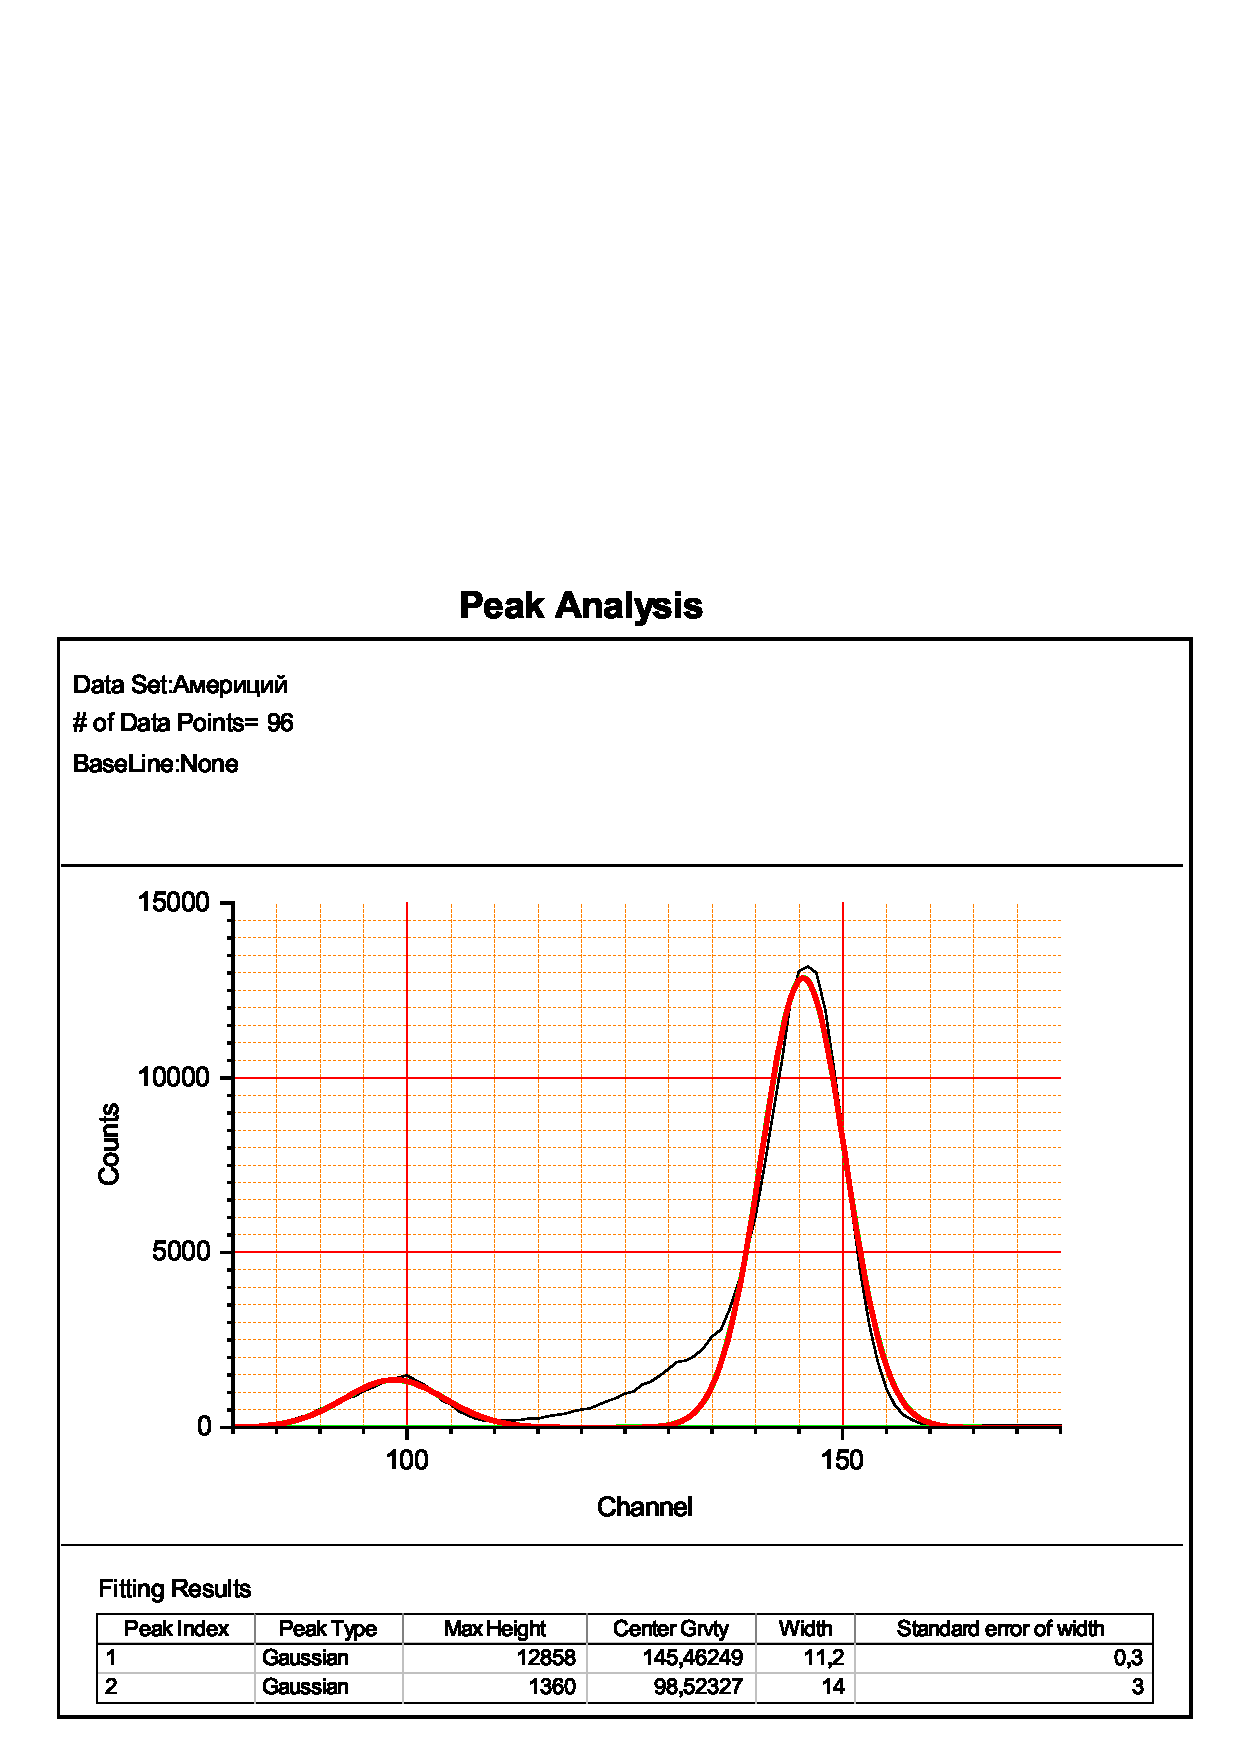
\includegraphics[width = \textwidth]{5.jpg}
\caption{График зависимости $\gamma_3$ от косинуса угла поляризации}
\end{center}
\end{figure}
\item Рассчитаем по формулам коэффициент и запишем все в таблицу 1. Затем представим все эти данные в графике (рис. 5). Все коэффициенты видности и $\delta$ рассчитаем по формулам $(12), (13), (14), (6)$

Все погрешности в таблицу берутся: для $\alpha$ --- половина цены деления, для $h_i \forall i \in {1, 2, 3, 4}$ так же половина цены деления, для $\gamma$ погрешность мы считаем, что 
\[\delta_{\gamma} = \gamma \cdot \sqrt{\left(\frac{2\delta_h}{h_4 - h_3}\right)^2 + \left(\frac{2\delta_h}{h_4 + h_3}\right)^2}\]
Она берется из того, что $\delta_{h_4 \pm h_3} = 2 \delta_h$. Так же возникает проблема в том, что если $h_4 = h_3$, то мы делим на 0, поэтому для этих случаев просто берем среднюю погрешность. Для $\delta$ берем погрешность 
\[\delta_{\delta} = \delta \cdot \sqrt{\left(\frac{\delta_{h}}{h_1}\right)^2 + \left(\frac{\delta_h}{h_2}\right)^2}\]
Для $\gamma_1$ берем погрешность 
\[\delta_{\gamma_1} = \gamma_1 \cdot \sqrt{ \left(\dfrac{\partial \gamma_1}{\partial \delta}\right)^2 \sigma_{\delta}^2} = \dfrac{2}{(1+\delta)^3}\cdot \sigma_{\delta}\]
\[\delta_{\gamma_2} = \gamma_2 \cdot \sqrt{\left(\frac{\delta_{\gamma}}{\gamma}\right)^2 + \left(\frac{\delta_{\gamma_1}}{\gamma_1}\right)^2}\]
\[\delta_{\gamma_3} = \gamma_3 \cdot \sqrt{\left(\frac{\delta_{\gamma}}{\gamma}\right)^2 + \left(\frac{\delta_{\gamma_1}}{\gamma_1}\right)^2}\]
\[\delta_{\cos\alpha} = \left| \sin \alpha \cdot \cos \alpha \right| \sigma_{\alpha}\]
\begin{table}[h!]
\begin{center}
\begin{tabular}{|c|c|c|c|c|c|c|c|c|c|c|c|c|}
\hline
$x$, см             & 10   & 12   & 14   & 16   & 18   & 20   & 22   & 21   & 24   & 26   & 28   & 30   \\ \hline
$\delta_x$, см      & 1    & 1    & 1    & 1    & 1    & 1    & 1    & 1    & 1    & 1    & 1    & 1    \\ \hline
$h_1$, ед           & 2,2  & 2,3  & 2,2  & 2,2  & 2,2  & 2,2  & 2,2  & 2,2  & 2,2  & 2,2  & 2,2  & 2,2  \\ \hline
$h_2$, ед           & 2,4  & 0,8  & 1,2  & 3,2  & 1,2  & 2,2  & 2,2  & 2,2  & 2    & 3,9  & 2    & 1    \\ \hline
$h_3$, ед           & 2,4  & 2,6  & 2,3  & 4,7  & 2,6  & 3,6  & 3,8  & 3,8  & 3,8  & 4,8  & 4,2  & 3,2  \\ \hline
$h_4$, ед           & 4    & 3,8  & 4,6  & 7    & 4,2  & 5,4  & 5,2  & 5,4  & 5    & 5,6  & 4,4  & 3,3  \\ \hline
$\delta_h$, ед      & 0,1  & 0,1  & 0,1  & 0,1  & 0,1  & 0,1  & 0,1  & 0,1  & 0,1  & 0,1  & 0,1  & 0,1  \\ \hline
$\delta$            & 0,92 & 0,35 & 0,55 & 1,45 & 0,55 & 1,00 & 1,00 & 1,00 & 0,91 & 0,56 & 0,91 & 0,45 \\ \hline
$\delta_{\delta}$   & 0,06 & 0,05 & 0,05 & 0,08 & 0,05 & 0,06 & 0,06 & 0,06 & 0,06 & 0,03 & 0,06 & 0,05 \\ \hline
$\gamma$            & 0,25 & 0,19 & 0,33 & 0,20 & 0,24 & 0,20 & 0,16 & 0,17 & 0,14 & 0,08 & 0,02 & 0,02 \\ \hline
$\delta_{\gamma}$   & 0,03 & 0,03 & 0,03 & 0,02 & 0,03 & 0,02 & 0,02 & 0,02 & 0,02 & 0,02 & 0,02 & 0,03 \\ \hline
$\gamma_1$          & 1,00 & 0,9  & 0,96 & 0,98 & 0,96 & 1,00 & 1,00 & 1,00 & 1,00 & 0,96 & 1,00 & 0,9  \\ \hline
$\delta_{\gamma_1}$ & 0,02 & 0,1  & 0,05 & 0,01 & 0,05 & 0,02 & 0,02 & 0,02 & 0,02 & 0,03 & 0,02 & 0,1  \\ \hline
$\gamma_2$          & 0,25 & 0,21 & 0,35 & 0,20 & 0,25 & 0,20 & 0,16 & 0,17 & 0,14 & 0,08 & 0,02 & 0,02 \\ \hline
$\delta_{\gamma_2}$ & 0,03 & 0,04 & 0,04 & 0,02 & 0,03 & 0,02 & 0,02 & 0,02 & 0,02 & 0,02 & 0,02 & 0,03 \\ \hline
\end{tabular}
\begin{tabular}{|c|c|c|c|c|c|c|c|c|c|c|c|c|}
\hline
$x$, см             & 34   & 36   & 38   & 42   & 46   & 50   & 54   & 56   & 58   & 60   & 62   & 64   \\ \hline
$\delta_x$, см      & 1    & 1    & 1    & 1    & 1    & 1    & 1    & 1    & 1    & 1    & 1    & 1    \\ \hline
$h_1$, ед           & 2,2  & 2,2  & 2,2  & 2,2  & 2,2  & 2,2  & 2,4  & 2,4  & 2,4  & 2,4  & 2,4  & 2,4  \\ \hline
$h_2$, ед           & 1,4  & 2    & 0,8  & 0,6  & 1,2  & 0,8  & 0,2  & 0,4  & 0,8  & 0,6  & 0,4  & 0,4  \\ \hline
$h_3$, ед           & 3,6  & 4,2  & 3    & 2,6  & 3,4  & 3    & 2,4  & 2,6  & 3    & 3    & 2,8  & 2,6  \\ \hline
$h_4$, ед           & 3,8  & 4,4  & 3,2  & 3,2  & 3,6  & 3    & 2,4  & 2,8  & 3,2  & 3    & 3    & 3    \\ \hline
$\delta_h$, ед      & 0,1  & 0,1  & 0,1  & 0,1  & 0,1  & 0,1  & 0,1  & 0,1  & 0,1  & 0,1  & 0,1  & 0,1  \\ \hline
$\delta$            & 0,64 & 0,91 & 0,36 & 0,27 & 0,55 & 0,36 & 0,08 & 0,17 & 0,33 & 0,25 & 0,17 & 0,17 \\ \hline
$\delta_{\delta}$   & 0,05 & 0,06 & 0,05 & 0,05 & 0,05 & 0,05 & 0,04 & 0,04 & 0,04 & 0,04 & 0,04 & 0,04 \\ \hline
$\gamma$            & 0,03 & 0,02 & 0,03 & 0,10 & 0,03 & 0,00 & 0,00 & 0,04 & 0,03 & 0,00 & 0,03 & 0,07 \\ \hline
$\delta_{\gamma}$   & 0,03 & 0,02 & 0,03 & 0,03 & 0,03 & 0,03 & 0,03 & 0,04 & 0,03 & 0,03 & 0,03 & 0,04 \\ \hline
$\gamma_1$          & 0,97 & 1,00 & 0,9  & 0,8  & 0,96 & 0,9  & 0,5  & 0,7  & 0,9  & 0,8  & 0,7  & 0,7  \\ \hline
$\delta_{\gamma_1}$ & 0,04 & 0,02 & 0,1  & 0,2  & 0,05 & 0,1  & 0,8  & 0,3  & 0,1  & 0,2  & 0,3  & 0,3  \\ \hline
$\gamma_2$          & 0,03 & 0,02 & 0,04 & 0,13 & 0,03 & 0,00 & 0,00 & 0,05 & 0,04 & 0,00 & 0,05 & 0,1  \\ \hline
$\delta_{\gamma_2}$ & 0,03 & 0,02 & 0,04 & 0,05 & 0,03 & 0,03 & 0,03 & 0,06 & 0,04 & 0,04 & 0,05 & 0,1  \\ \hline
\end{tabular}
\begin{tabular}{|c|c|c|c|c|c|c|c|c|c|c|c|c|}
\hline
$x$, см             & 66   & 68   & 70   & 72   & 74   & 76   & 78   & 80   & 82   & 84   & 86   & 88   \\ \hline
$\delta_x$, см      & 1    & 1    & 1    & 1    & 1    & 1    & 1    & 1    & 1    & 1    & 1    & 1    \\ \hline
$h_1$, ед           & 2,4  & 2,4  & 2,4  & 2,4  & 2,4  & 2,5  & 2,8  & 2,4  & 3,2  & 3,4  & 3,4  & 3,4  \\ \hline
$h_2$, ед           & 0,4  & 0,8  & 0,4  & 0,6  & 0,8  & 1    & 1,2  & 2,4  & 1,6  & 1    & 1,6  & 2,2  \\ \hline
$h_3$, ед           & 2,6  & 2,8  & 2,8  & 2,6  & 2,6  & 2,7  & 3,2  & 3,6  & 4,4  & 4    & 4,6  & 3,4  \\ \hline
$h_4$, ед           & 3,2  & 3,4  & 3,2  & 3,7  & 4    & 4,3  & 4,6  & 5,7  & 5,2  & 4,8  & 5,2  & 4    \\ \hline
$\delta_h$, ед      & 0,1  & 0,1  & 0,1  & 0,1  & 0,1  & 0,1  & 0,1  & 0,1  & 0,1  & 0,1  & 0,1  & 0,1  \\ \hline
$\delta$            & 0,17 & 0,33 & 0,17 & 0,25 & 0,33 & 0,40 & 0,43 & 1,00 & 0,50 & 0,29 & 0,47 & 0,65 \\ \hline
$\delta_{\delta}$   & 0,04 & 0,04 & 0,04 & 0,04 & 0,04 & 0,04 & 0,04 & 0,06 & 0,03 & 0,03 & 0,03 & 0,04 \\ \hline
$\gamma$            & 0,10 & 0,10 & 0,07 & 0,17 & 0,21 & 0,23 & 0,18 & 0,23 & 0,08 & 0,09 & 0,06 & 0,08 \\ \hline
$\delta_{\gamma}$   & 0,03 & 0,03 & 0,03 & 0,03 & 0,03 & 0,03 & 0,03 & 0,02 & 0,02 & 0,02 & 0,02 & 0,03 \\ \hline
$\gamma_1$          & 0,7  & 0,9  & 0,7  & 0,8  & 0,9  & 0,9  & 0,9  & 1,00 & 0,94 & 0,8  & 0,93 & 0,98 \\ \hline
$\delta_{\gamma_1}$ & 0,3  & 0,1  & 0,3  & 0,2  & 0,1  & 0,1  & 0,1  & 0,01 & 0,04 & 0,1  & 0,04 & 0,02 \\ \hline
$\gamma_2$          & 0,1  & 0,11 & 0,1  & 0,2  & 0,24 & 0,25 & 0,20 & 0,23 & 0,09 & 0,11 & 0,07 & 0,08 \\ \hline
$\delta_{\gamma_2}$ & 0,1  & 0,04 & 0,1  & 0,1  & 0,05 & 0,04 & 0,03 & 0,02 & 0,02 & 0,03 & 0,02 & 0,03 \\ \hline
\end{tabular}
\caption{Входные данные и все, что из них получено для зависимости от $x$ всех величин.}
\end{center}
\end{table}
\item Исследуйте зависимость видности от разности хода между лучами. Для этого установите поляроид П1 в положение, в котором интерференционная картина видна наиболее чётко. И исследуем зависимость $h_i$ от координаты $x$.
\item Рассчитаем коэффициент $\gamma_2$ по формулам и построим график.

Определим по нему $l_{1/2}$, $L$ и $\Delta \nu$
Из установки мы видим, что $L = 65 cm$, $\lambda = 632,8 nm$.

Из графики видим, что $l_{1/2} \approx (4,8 \pm 0,3)$ см, отсюда из формулы $(16)$ можем найти 
\[\Delta F \approx \frac{0,26 c}{l_{1/2}} \approx (1,5 \pm 0,1) \cdot 10^9 \text{Гц}\]
\[\Delta \nu = \frac{c}{2L} = (2,5 \pm 0,2) \cdot 10^8 \text{Гц}\]
Что примерно соответствует теоретическим предположениям о том, что $\Delta F \sim 10^9 \div 10^10$ Гц. 

Теперь по формуле $(4)$ мы можем найти 
\[N \approx 1 + \frac{2 \cdot 1,5 \cdot 10^9}{2,5 \cdot 10^8} \approx 7 \]

Погрешности находим по формулам, для $l_{1/2}$ находим для 2 разных пиков и усредняем. Для $\Delta F$ по формуле 
\[\delta_{\Delta F} = \Delta F \cdot \frac{\delta_{l_{1/2}}}{l_{1/2}}\]
\[\delta_{\Delta \nu} = \Delta \nu \cdot \frac{\delta_L}{L}\]
\[\delta_N = N \cdot \sqrt{\left( \frac{\delta_{\Delta F}}{\Delta F}\right)^2 + \left( \frac{\delta_{\Delta \nu}}{\Delta \nu}\right)^2}\]
Видим, что $\delta_N \approx 0,4$ а поскольку мы знаем, что $N$ целое, то можно утверждать что $N = 7$ без погрешности. 
\begin{figure}[h]
\begin{center}
\includegraphics[width = \textwidth]{6.jpg}
\caption{График зависимости $\gamma_2$ от $x$}
\end{center}
\end{figure}
\end{enumerate}
\newpage
\section*{Вывод}
При изучении зависимости от угла поляризации $\gamma_3$ мы видим, что график зависимости $\gamma_3$ похож на график модуля $\cos \alpha$, однако умноженный на коэффициент примерно $\frac{1}{2}$. Это может быть связано с тем, что максимум $\gamma_2(x)$ примерно на 16 см. Однако мы могли установить не совсем на 16 см. В итоге мы получаем, что $gamma_2 = \frac{1}{2}$, что мы и видим.

При изучении зависимости от $x$, мы видим, что пики на расстоянии между ними $62$ см. Что почти равно настоящему значению, а именно $65$ см.
\end{document}